\seccion{Entrop\'ia condicional, informaci\'on mutua, entrop\'ia relativa}
\label{Sec:SZ:Mutua}

Tratando de un par de variables aleatorias $X$ e $Y$, una cuesti\'on natural que
ocurre  es de  cuantificar la  incerteza que  queda sobre  una de  las variables
cuando se  observa la otra.   Dicho de otra  manera, si se  mide $Y =  y$, ?`que
informaci\'on lleva sobre  $X$? La respuesta a esta  interogaci\'on se encuentra
en la noci\'on de entrop\'ia condicional.  Si uno mide $Y = y$, la descripci\'on
estad\'istica  de $X$  conociendo este  $Y =  y$ se  resuma a  la distribuci\'on
condicional de probabilidad  $p_{X|Y=y} = \frac{p_{X,Y}(\cdot,y)}{p_Y(y)}$.  Con
esta  restricci\'on, se  puede evaluar  una  incerteza sobre  $X$, sabiendo  que
$Y=y$,
%
\[
H(X|Y=y) = H\left( p_{X|Y=y} \right).
\]
%
Entonces, condicionalmente a la variable aleatoria $Y$, la incerteza va a ser el
promedio  estad\'istico sobre  todos  los estados  $Y$  es decir  $\displaystyle
H(X|Y)  = \int_{\Rset^d}  p_Y(y) H(X|Y=y)  \, d\mu(y)$  \ (con  la  medida $\mu$
adecuada).
%
\begin{definicion}[Entrop\'ia condicional]
\label{Def:SZ:entropiacondicional}
%
  Sean \ $X$ \ e \ $Y$ \ dos variables aleatorias, respectivamente \ $d$ \ y \
  $d'$-dimensionales. La entrop\'ia condicional de  \ $X$, con respeto a \ $Y$,
  es definida por
  %
  \[
  H(X|Y)   =   -  \int_{\Rset^d   \times   \Rset^{d'}}  p_{X,Y}(x,y)   \log
  p_{X|Y=y}(x) \, d\mu(x,y),
  \]
  %
  con \ $\mu$ \ medida adecuada (ej.  discreta en el caso discreto o de Lebesgue
  en el caso diferencial).
\end{definicion}

Si  $X$ e  $Y$ son  independientes,  $p_{X|Y=y}$ se  reduce a  $p_X$, as\'i  que
obviamente,
%
\begin{propiedades}
\item\label{Prop:SZ:independenciacondicional}
  %
  \[
  X \: \mbox{e} \: Y \: \mbox{independientes} \quad \Leftrightarrow \quad H(X|Y)
  = H(X).
  \]
\end{propiedades}
%
Esta  propiedad  se   interpreta  como  el  hecho  que   $Y$  no  lleva  ninguna
informaci\'on sobre  $X$, y entonces ninguna  medici\'on de $Y$ va  a cambiar la
incerteza sobre $X$.

Siendo $H(X|Y=y)$  una entrop\'ia, va a  heredar de todas las  propiedades de la
entrop\'ia  (o  entrop\'ia   diferencial).   Adem\'as,  de  $p_{X,Y}(\cdot,y)  =
p_{X|Y=y} p_Y(y)$ se deduce la propiedad siguiente
%
\begin{propiedades}
\item\label{Prop:SZ:cadena}  {\it Regla de  cadena}
  %
  \[
  H(X,Y) =  H(X|Y) +  H(Y).
  \]
  %
  Esta regla se generaliza sencillamente a
  %
  \[
  H(X_1 , \ldots , X_n) = H(X_1) + \sum_{i=2}^n H(X_i|X_{i-1} , \ldots , X_1).
  \]
  %
  De       esta       regla      de       cadena       se      recupera       la
  propiedad~\ref{Prop:SZ:independenciacondicional}     a     partir    de     la
  propiedad~\ref{Prop:SZ:aditividad}.
\end{propiedades}
%
Siendo  $H(X|Y=y)$  una  entrop\'ia,  en  el  caso  discreto  esta  cantidad  es
positiva. Entonces, en el caso discreto,  $H(X|Y)$ es positiva, lo que prueba la
super-aditividad~\ref{Prop:SZ:superaditividad}.

De la regla de  cadena $H(X,Y) = H(X|Y) + H(Y) = H(Y|X)  + H(X)$ aparece que las
cantidades \ $H(X|Y)-H(X)$, \  $H(Y|X)-H(Y)$ \ y \ $H(X,Y) - H(X)  - H(Y)$ \ son
todas iguales. Estas  cantidades definen lo que se  llama la informaci\'on mutua
entre \ $X$ \ e \ $Y$:

\begin{definicion}[Informaci\'on mutua]
\label{Def:SZ:mutua}
%
  Sean $X$ e $Y$ dos variables  aleatorias, la informaci\'on mutua entre \ $X$ \
  e  \ $Y$ \  es la  cantidad sim\'etrica
  %
  \[
  I(X;Y) = H(X|Y)-H(X) = H(Y|X)-H(Y) = H(X,Y) - H(X) - H(Y);
  \]
  %
  Se expresa
  %
  \[
  I(X;Y)  =  \int_{\Rset^d  \times  \Rset^{d'}}  p_{X,Y}(x,y)  \log  \left(
    \frac{p_{X,Y}(x,y)}{p_X(x) p_Y(y)} \right) \, d\mu(x,y)
  \]
  %
  con \ $\mu$ \  medida adecuada (discreta en el caso discreto  o de Lebesgue en
  el caso diferencial).
\end{definicion}

Las  diferentes  cantidades  pueden  ser  vistas  a  trav\'es  de  una  visi\'on
ensemblista, como descrita en la figura Fig.~\ref{Fig:SZ:Venn}, diagrama de Venn
o de Euler (ver nota de pie~\ref{Foot:MP:Euler}.
% pagina~\pageref{Foot:MP:Euler}.

\begin{figure}[h!]
%
\begin{center} 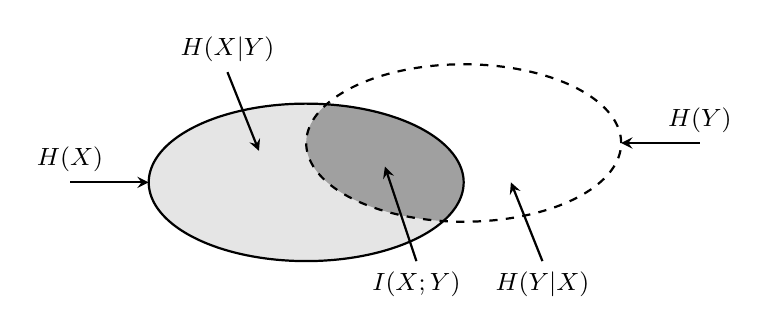
\begin{tikzpicture}[scale=2]
\shorthandoff{>}
% interior H(X) x^2 + 4 y^2 = 1 => y = \pm sqrt(1-x^2)/2
\fill[domain=0:360,samples=200,opacity=.1] plot ({cos(\x)},{.5*sin(\x)});
%
% interior H(Y) (x-1)^2 + 4 (y-1/4)^2 = 1 => y = 1/4 \pm sqrt(1-(x-1)^2)/2
% se cruzan cuando x = 1 \pm sqrt(55)/10 =>
% theta = acos(.5 \pm sqrt(55)/20) para X
% theta = acos(-.5 \pm sqrt(55)/20) para X
\pgfmathsetmacro{\s}{acos(.5-sqrt(55)/20)};
\pgfmathsetmacro{\t}{-acos(.5+sqrt(55)/20)};
\pgfmathsetmacro{\u}{-acos(-.5+sqrt(55)/20)};
\pgfmathsetmacro{\v}{acos(-.5-sqrt(55)/20)-360};
%
% interior I(X;Y)
%\draw[domain=\v:\v] plot ({cos(\x)+1},{.5*sin(\x)+.25}) node{$\bullet$};
\fill[opacity=.3]
   plot [domain=\s:\t,samples=200] ({cos(\x)},{.5*sin(\x)})
-- plot [domain=\u:\v,samples=200] ({cos(\x)+1},{.5*sin(\x)+.25})
-- cycle;
%
% borders H(X) y H(Y)
\draw[domain=0:360,samples=200,thick] plot ({cos(\x)},{.5*sin(\x)});
\draw[dashed,domain=0:360,samples=200,thick] plot ({cos(\x)+1},{.5*sin(\x)+.25});
%
% flechas y flechas condicionales
\draw[thick,>=stealth,<-] (-1,0)--(-1.5,0) node[above]{\small $H(X)$};
\draw[thick,>=stealth,<-] (-.3,.2)--(-.5,.7) node[above]{\small $H(X|Y)$};
%
\draw[thick,>=stealth,<-] (2,.25)--(2.5,.25) node[above]{\small $H(Y)$};
\draw[thick,>=stealth,<-] (1.3,0)--(1.5,-.5) node[below]{\small $H(Y|X)$};
%
\draw[thick,>=stealth,<-] (.5,.1)--(.7,-.5) node[below]{\small $I(X;Y)$};
\end{tikzpicture} \end{center}
%
\leyenda{Diagrama  de Venn: Ilustraci\'on  de la  definici\'on de  la entrop\'ia
  condicional, de la informaci\'on mutua, y de las relaciones entre cada medida.
  La superficia del  elipse en linea llena (parte grise)  representa $H(X)$ y el
  interior de la  en linea discontinua representa $H(Y)$.   La parte grise clara
  representa $H(X|Y)$  superficia del ``conjunto $H(X)$'' quitando  la parte que
  partenece  a  $H(Y)$.  La  parte  blanca  representa  $H(Y|X)$ superficia  del
  ``conjunto $H(Y)$''  quitando la  parte que partenece  a $H(X)$.  La  parte en
  grise oscuro es entonces lo que $X$ e $Y$ comparten, es decir $I(X;Y)$.}
%
\label{Fig:SZ:Venn}
\end{figure}

Como se lo va a probar, $I$ es positiva; representa realmente una informaci\'on,
la compartida  entre \ $X$  \ e  \ $Y$: Si  de la incerteza  de $X$ se  quita la
incerteza  de  $X$   una  vez  que  $Y$  es  medida,  lo   que  queda  tiene  la
significaci\'on de  la informaci\'on que  estas variables tienen en  com\'un. En
particular, de $I(X;X) = H(X)$ se denoma a veces $H(X)$ {\it auto informaci\'on}
de $X$.

Para  probar la  positividad de  $I$, se  introduce de  manera m\'as  general la
noci\'on  de  entrop\'ia  relativa,   conocida  tambi\'en  como  divergencia  de
Kullback-Leibler~\cite{KulLei51, Kul68, CovTho06, Rio07}:
%
\begin{definicion}[Entrop\'ia relativa]
\label{Def:SZ:entropiarelativa}
%
La entrop\'ia  relativa, o  divergencia de una  medida de probabilidad  $Q$, con
respeto a una medida de probabilidad de referencia $P$ tal que \underline{$Q \ll
  P$}, ambas definidas sobre $\Rset^d$, es definida como
  %
  \[
  \Dkl[Q]{P}  =  \int_{\Rset^d}  \frac{dQ}{dP}(x) \, \log  \left(  \frac{dQ}{dP}(x)
  \right)  \, dP(x)  = \int_{\Rset^d}  \log \left(  \frac{dQ}{dP}(x)  \right) \,
  dQ(x).
  \]
  %
  Si \  $P$ \  y \ $Q$  \ admiten una  densidad con  respeto a una  medida $\mu$
  (basicamente nos interesamos  a $\mu_L$ y $\mu_\X$), se  escribe a trav\'es de
  las  densidades  como~\footnote{En el  caso  discreto,  esta cantidad  depende
    solamente de $p$ y $q$ y no  de los estados. La condici\'on necesaria es que
    $p$ y $q$ tienen los mismos  n\'umeros de componentes (se completa el vector
    lo m\'as corto)  y si la $i$-esima componente de $q$  vale cero, entonces la
    de $p$ vale  cero tambi\'en.  Adem\'as, con $p$ y $q$  de mismo tama\~no, se
    puede poner en biyecci\'on los alfabetos  asociados a $p$ y $q$, sin perdida
    de generalidad.  En el caso  continuo, esta razonamiento no vale m\'as, esta
    cantidad dependiendo en general de los estados\ldots}
  %
 \[
 \Dkl[q]{p}  \equiv \Dkl[Q]{P}  = \int_{\Rset^d}  \log  \left( \frac{q(x)}{p(x)}
 \right) \, q(x) \, d\mu(x).
 \]
  %
\end{definicion}
%
Inicialmente, esta  medida fue  introducida por Kullback  y Leibler en  la misma
linea  que Shannon, interpretando  \ $\log\left(\frac{dQ}{dP}(x)\right)$  \ como
una informaci\'on de discriminaci\'on  entre dos hip\'otesis de distribuciones \
$Q$ \ y \  $P$ \ a partir de la observaci\'on \ $x$,  \ la divergencia siendo la
informaci\'on   de  discriminaci\'on   promedia.   Introdujeron   tambi\'en  una
versi\'on sim\'etrica, que veremos m\'as adelante.  Se notar\'a que, $\Dkl[Q]{P}
=  - \int_{\Rset^d}  q(x)  \, \log(q(x))  \,  d\mu(x) +  \int_{\Rset^d} p(x)  \,
\log(q(x)) \, d\mu(x)$.  El primer termino es nada mas que la entrop\'ia de $q$,
que se puede  ver como distribuci\'on ``presupuesta''. Menos  el secundo termino
se interpreta como el promedio de la incerteza elemental $\log(q)$ con respeto a
la distribuci\'on de referencia (``verdadera''), a veces llamado {\it entrop\'ia
  cruzada}.   Por eso,  esta divergencia  es una  entrop\'ia relativamente  a la
distribuci\'on  $p$.  En  la  misma linea,  se  puede inmediatamente  ver de  la
definici\'on general Def.~\ref{Def:SZ:ShanonMu},
%pagina~\pageref{Def:SZ:ShanonMu}, 
que  $\displaystyle  \Dkl[Q]{P} \equiv  -H\left(  \frac{dQ}{dP}  \right)$ \  con
respeto a la medida $\mu = P$.   Por ejemplo, en el caso discreto finito, si $p$
es  la   distribuci\'on  uniforme  sobre  un  alfabeto   de  cardinal  $\alpha$,
$\Dkl[q]{p} =  \log \alpha  - H(q)$,  lo que representa  una desviaci\'on  de la
entrop\'ia de  su valor  m\'aximo.  La misma  interpretaci\'on queda en  el caso
continuo con  la ley  uniforme ($p$ y  $q$ definidas  sobre el mismo  espacio de
volumen  finito) o  con la  gaussiana ($p$  y $q$  teniendo la  misma  matriz de
covarianza).  {\it Como para la  entrop\'ia, cuando se necesitar\'a un logaritmo
  especificamente de base $a$, se notar\'a la divergencia $D_{\mathrm{kl},a}$.}

\begin{lema}[Positividad de la entrop\'ia relativa]
\label{Lem:SZ:PositividadEntropiaRelativa}
%
  \[
  \Dkl[Q]{P} \ge 0 \quad \mbox{con igualdad ssi} \quad P = Q. %\quad (c.s.)
  \]
  %
\end{lema}
%
\begin{proof}
  Existen varias pruebas, pero la m\'as linda puede ser la usando la desigualdad
  de  Jensen~\footnote{En   el  caso  discreto,  se  puede   usar  tambi\'en  la
    desigualdad \ $\sum t_i \log t_i \ge  \sum t_i \log t'_i$ \ una instancia de
    la desigualdad conocida como  desigualdad log-sum, o conocida tambi\'en como
    desigualdad de  Gibbs (debido a J.  W.   Gibbs mismo)~\cite{Gib02, CovTho06,
      Rio07,         Mer10,        Mer18}.},        teorema~\ref{Teo:MP:Jensen}:
  %pagina~\pageref{Teo:MP:Jensen}:  
  para $\phi$ convexa  e \ $Y$ \ variable  aleatoria escalar, $\Esp[\phi(Y)] \ge
  \phi(\Esp[Y])$ \ con igualdad ssi \  $Y$ \ es determinista (casi siempre) si \
  $\phi$ es estrictamente  convexa.  Sea \ $X$ \ de  medida de probabilidad $P$.
  Se escribe la entrop\'ia  relativa \ $\Dkl[Q]{P} = \Esp\left[ \frac{dQ}{dP}(X)
    \log \left( \frac{dQ}{dP}(X) \right) \right]$.  Sea \ $Y = \frac{dQ}{dP}(X)$
  y  $\phi(u)  =  u  \log  u$,  funci\'on  estrictamente  convexa.   Entonces  \
  $\Dkl[Q]{P}  =  \Esp[\phi(Y)] \ge  \phi(\Esp[Y])$.   \  Pero \  $\displaystyle
  \Esp[Y]    =   \Esp\left[    \frac{dQ}{dP}(X)    \right]   =    \int_{\Rset^d}
  \frac{dQ}{dP}(x)       \,       dP(x)        =       1$       seg\'un       el
  lema~\ref{Lem:RelacionIntegracionDerivadasRadon}.
  %pagina~\pageref{Lem:RelacionIntegracionDerivadasRadon}.  \ 
  Se cierra  la prueba  con el hecho  que \  $\phi(1) = 0$  El caso  de igualdad
  apareciendo  si   y  solamente   si  \  $Y$   \  es  determinista,   es  decir
  $\frac{dP}{dQ}(X)$ \ determinista, es equivalente a \ $\frac{dP}{dQ} = 1 \quad
  (P$-c.s.)    \    (constante,   la   constante   siendo   igual    a   1   del
  lema~\ref{Lem:RelacionIntegracionDerivadasRadon} y  \ $P$ \  y \ $Q$  \ siendo
  medidas de probabilidad).
\end{proof}

Esta propiedad tiene consecuencias fijandose que
%
\[
I(X;Y) = \Dkl[P_{X,Y}]{P_X P_Y},
\]
%
\ie  la  informaci\'on  mutua  es  la  divergencia  de  Kullback-Leibler  de  la
distribuci\'on  conjunta  relativa al  producto  de  las marginales  (obviamente
$P_{X,Y} \ll  P_X P_Y$). Con este  enfoque, no se  necesita que \ $(X,Y)$  \ sea
discreta o continua admitiendo una densidad.
%
\begin{propiedades}
\item\label{Prop:SZ:Ipositive}   {\it   $I$   es   positiva,  como   medida   de
    independencia:}
  %
  \[
  I(X;Y) \ge 0 \quad \mbox{con igualdad ssi $X$ e $Y$ son independientes.}
  \]
%
\item\label{Prop:SZ:condicionar} {\it  Condicionar reduce la  entrop\'ia}
  %
  \[
  H(X|Y) \le H(X) \quad \mbox{con igualdad ssi $X$ e $Y$ son independientes.}
  \]
  %
  Esta    desigualdad,     con    la     regla    de    cadena,     prueba    la
  sub-aditividad~\ref{Prop:SZ:subaditividad}.   Esta  reducci\'on  de  incerteza
  vale en  promedio, pero el conocimiento  de un valor particular  puede ser tal
  que $H(X|Y =  y) > H(X)$, \ie \ !`un conocimiento  particular puede aumentar la
  entrop\'ia!  (ver ejemplos en~\cite[p.~59]{Rio07}).
\end{propiedades}

Fijense  que   si  $\Dkl{}$  es   positiva,  \underline{no  es   sim\'etrica}  y
\underline{tampoco  satisface la  desigualdad triangular}.  Por eso,  no  es una
distancia  y  tiene  el  nombre  de {\it  divergencia}.   La  distribuci\'on  de
referencia $P$ juega un rol fundamental.

Al  final, se mencionar\'a las propiedades adicionales siguientes:
%
\begin{enumerate}
\item $\Dkl[q]{p}$  queda invariante  bajo una misma  transformaci\'on biyectiva
  sobre  ambos $p$ y  $q$. Es  trivial en  el caso  discreto y  si no  se prueba
  sencillamente por un cambio de variables en la forma integral.
%
\item $\Dkl{}$  es convexa con respecto al  par $(P,Q)$ en el  sentido que, para
  $\pi_i \ge 0,  \: \sum_i \pi_i = 1$,  y dos conjuntos $\{ P_{(i)}  \}_i, \: \{
  Q_{(i)} \}_i$ de medidas de probabilidades tales que $Q_{(i)} \ll P_{(i)}$,
  %
  \[
  \Dkl[\sum_i   \pi_i  \ Q_{(i)}]{\sum_i   \pi_i \   P_{(i)}}  \ge   \sum_i   \pi_i
  \Dkl[Q_{(i)}]{P_{(i)}}.
  \]
  %
  La  prueba de  esta desigualdad  es dada  subsecci\'on~\ref{Ssec:SZ:Csiszar}
  %, pagina~\pageref{Ssec:SZ:Csiszar} 
  en un contexto m\'as general.
%
\item Para  $Q$ fijo, $\Dkl[Q]{P}$ es convexa  con respecto a $P$  en el sentido
  que, para $\pi_i \ge 0, \: \sum_i  \pi_i = 1$, y un conjunto $\{ P_{(i)} \}_i$
  de medidas de probabilidades tales que $Q \ll P_{(i)}$,
  %
  \[
  \Dkl[Q]{\sum_i   \pi_i \,   P_{(i)}}  \ge   \sum_i   \pi_i
  \, \Dkl[Q]{P_{(i)}}.
  \]
  %
  Eso  es  la  consecuencia  obvia  de  la concavidad  de  $u  \mapsto  \log  u$
  (escribiendo la divergencia  como densidad con respeto a  una medida dada). Es
  sencillo ver que si $\Dkl{}$ siendo convexa con respecto a $P$ ($Q$ dada) y al
  par $(P,Q)$, no puede ser convexa con respecto a $Q$ (con $P$ dada).
\end{enumerate}
